\documentclass[arhiv]{izpit}
\usepackage{fouriernc}
\usetikzlibrary{calc}
\renewcommand{\ttdefault}{txtt}

\begin{document}

\izpit{Programiranje I: 3.~izpit}{6.~september 2013}{
  Čas reševanja je 120 minut.
  Veliko uspeha!
}

%%%%%%%%%%%%%%%%%%%%%%%%%%%%%%%%%%%%%%%%%%%%%%%%%%%%%%%%%%%%%%%%%%%%%%
\naloga[30 točk]

Pravimo, da je vrednost nekega vozlišča v dvojiškem drevesu \emph{lokalni minimum},
  če je manjša ali enaka vrednostim v vseh sosednjih vozliščih.
Na primer, v drevesu
%
\[
  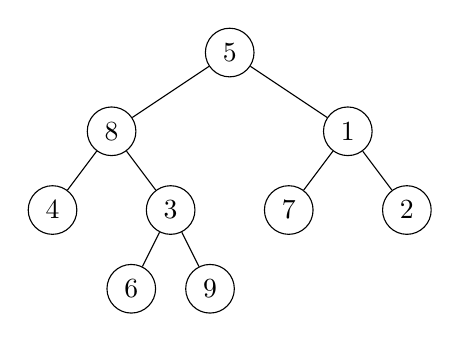
\begin{tikzpicture}[level distance=1cm,
    level 1/.style={sibling distance=3cm},
    level 2/.style={sibling distance=1.5cm},
    level 3/.style={sibling distance=1cm}
    ]
    \node[circle, draw] (d) {5}
      child {node[circle, draw] {8}
        child {node[circle, draw] {4}}
        child {node[circle, draw] {3}
          child {node[circle, draw] {6}}
          child {node[circle, draw] {9}}
        }
      }
      child {node[circle, draw] {1}
        child {node[circle, draw] {7}}
        child {node[circle, draw] {2}}
      };
  \end{tikzpicture}
\]
%
so lokalni minimumi števila $1$, $3$ in $4$.

Razredu \verb|Drevo| dodajte metodo \verb|naloga1(self)|,
  ki v času $O(h)$, kjer je $h$ višina drevesa,
  poišče en (katerikoli) lokalni minimum.
Če lokalnega minimuma ni, naj metoda vrne \verb|None|.


%%%%%%%%%%%%%%%%%%%%%%%%%%%%%%%%%%%%%%%%%%%%%%%%%%%%%%%%%%%%%%%%%%%%%%
\naloga[30 točk]

Dana naj bo matrika $(a_{i,j})_{i,j} \in \mathbb{R}^{m \times n}$,
  v kateri so elementi razporejeni tako, da so vse vrstice naraščajoče,
  vsi stolpci pa padajoči, na primer:
%
\[
  \begin{bmatrix}
    3 & 5 & 7 & 9 \\
    2 & 4 & 5 & 8 \\
    1 & 3 & 4 & 5
  \end{bmatrix}
\]
%
Natančneje torej velja $a_{i,j} < a_{i,j+1}$ za vse $1 \le i \le m$ in $1 \le j < n$,
ter $a_{i,j} > a_{i+1,j}$ za vse $1 \le i < m$ in $1 \le j \le n$.

Sestavite funkcijo \verb|naloga2(a, x)|, ki vrne \verb|True|, kadar
  se število \verb|x| pojavi v matriki \verb|a|, in \verb|False| sicer.
{\small\begin{verbatim}
   >>> a = [[3, 5, 7, 9], [2, 4, 5, 8], [1, 3, 4, 5]]
   >>> naloga2(a, 7)
   True
   >>> naloga2(a, 2)
   True
   >>> naloga2(a, 6)
   False\end{verbatim}}
Časovna zahtevnost funkcije naj bo $O(m + n)$, kjer je $m \times n$ velikost matrike \verb|a|.


%%%%%%%%%%%%%%%%%%%%%%%%%%%%%%%%%%%%%%%%%%%%%%%%%%%%%%%%%%%%%%%%%%%%%%
\naloga[40 točk]

Zaporedje točk v ravnini
\[
  (x_1, y_1), (x_2, y_2), \dots, (x_n, y_n)
\]
imenujemo \emph{pravokotni celoštevilski sprehod},
kadar so vse koordinate celoštevilske,
za vsaki dve zaporedni točki pa velja
bodisi $x_i = x_{i + 1}$ bodisi $y_i = y_{i + 1}$.
Na vsakem koraku se torej premaknemo bodisi vodoravno bodisi navpično.

Pravimo, da je pravokotni celoštevilski sprehod \emph{naraščajoč},
kadar za vsaki dve zaporedni točki velja
$x_i \le x_{i + 1}$ in $y_i \le y_{i + 1}$.
Na vsakem koraku se torej premaknemo bodisi desno bodisi navzgor.

\podnaloga
V \emph{Mathematici} sestavite funkcijo \verb|naloga3a[sez_]|,
ki sprejme seznam celoštevilskih točk v ravnini \verb|sez| in
nariše te točke ter pravokotni celoštevilski sprehod,
ki jih zaporedoma obhodi.

Možnih pravokotnih celoštevilskih sprehodov skozi dane točke je neskončno
in vseeno je, katerega izmed njih narišete.

\begin{center}
  \includegraphics[width=0.3\textwidth]{sprehod3a.pdf} \\
  \verb|naloga3a[{{0, 0}, {3, 3}, {2, 0}, {1, 2}}]|
\end{center}

\podnaloga
V \emph{Mathematici} sestavite funkcijo \verb|naloga3b[zac_, sez_, kon_]|,
ki nariše \emph{naraščajoči} pravokotni celoštevilski sprehod,
ki se začne v točki \verb|zac|, konča v točki \verb|kon|
in se v celoti izogne vsem točkam iz seznama \verb|sez|.

Zopet je vseeno, katerega izmed možnih sprehodov narišete,
predpostavite pa lahko, da obstaja vsaj eden.

\begin{center}
  \includegraphics[width=0.3\textwidth]{sprehod3b.pdf} \\
  \verb|naloga3b[{0, 0}, {{0, 2}, {2, 1}, {1, 3}}, {3, 3}]|
\end{center}

\end{document}

